\begin{figure}[h]
 \centering
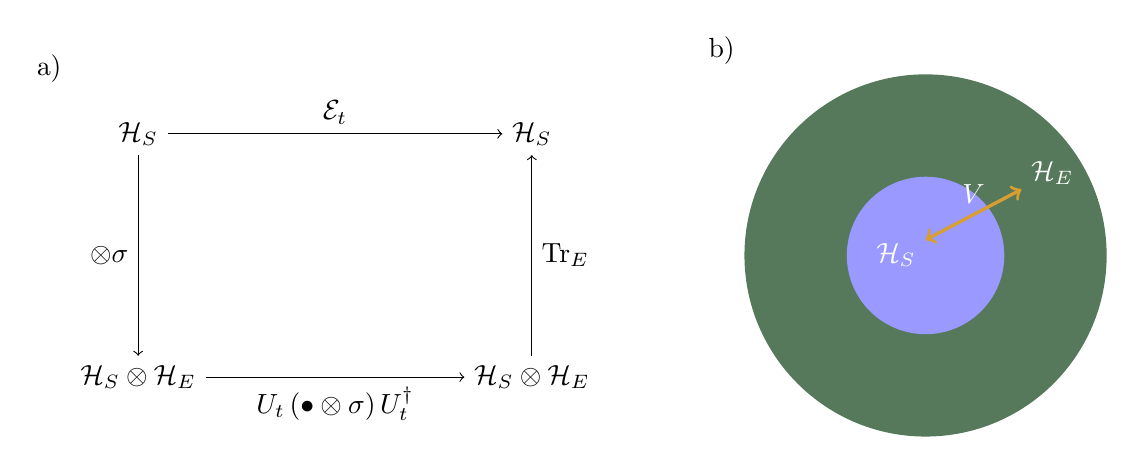
\begin{tikzpicture}%[transform canvas={scale=1.3}]
% Define colors
\definecolor{colorenv}{HTML}{55795A}
\definecolor{colorsys}{HTML}{7286D3}
\definecolor{colorarrow}{HTML}{D99E30}
  %%%%%%%%%%%%%%%%%5Commutation diagram
  % Define nodes
  \begin{scope}[local bounding box=drawA]
  \node (A) at (0cm,0) {$\mathcal{H}_{S}$};
   \node (B) at (5cm,0) {$\mathcal{H}_{S}$};
  \node (C) at (0cm,-3.09cm) {$\mathcal{H}_{S}\otimes\mathcal{H}_{E}$};
  \node (D) at (5cm,-3.09cm) {$\mathcal{H}_{S}\otimes\mathcal{H}_{E}$};
  % Draw arrows
   \draw[->] (A) -- (B) node[midway, above] {$\mathcal{E}_{t}$};
  \draw[->] (A) -- (C) node[midway, left] {$\otimes \sigma$};
  \draw[<-] (B) -- (D) node[midway, right] {$\mathrm{Tr}_{E}$};
  \draw[->] (C) -- (D) node[midway, below] {$U_{t}\left(\bullet\otimes\sigma\right)U_{t}^{\dagger}$};
\end{scope}
\node[above left] at (drawA.north west) {a)};
  \begin{scope}[local bounding box=drawB]
  %%%%%%%%%%The circles
  %Circles
  \fill[color=colorenv] (10cm,-1.545cm) circle (2.3cm);

  \fill[blue!40] (10cm,-1.545cm) circle (1cm);
  %Marks
  \node[text=white, anchor=east] (E) at (10cm,-1.545cm) {$\mathcal{H}_{S}$};
  \node[text=white, anchor=east] (F) at (12cm,-0.5cm) {$\mathcal{H}_{E}$};
   \draw[<->, line width=1.2pt, color=colorarrow, text=white] (E) -- (F) node[midway, above] {$V$};
  \end{scope}
 \node[above left] at (drawB.north west) {b)};
\end{tikzpicture}
\caption{Diagrams of the $S+E$ scheme. In a) the maps that define $\mathcal{E}_{t}$ are shown, and in b) a Venn-like diagram illustrating
the structure of the total system $S+E$, inspired in \cite{manzano2020short} }
\label{fig:SE_Diagrams}
\end{figure}
